\section{Initial Central-Setting Comparisons}
\label{app:initial-central}
\par\medskip\noindent\begin{minipage}{\linewidth}

\centering
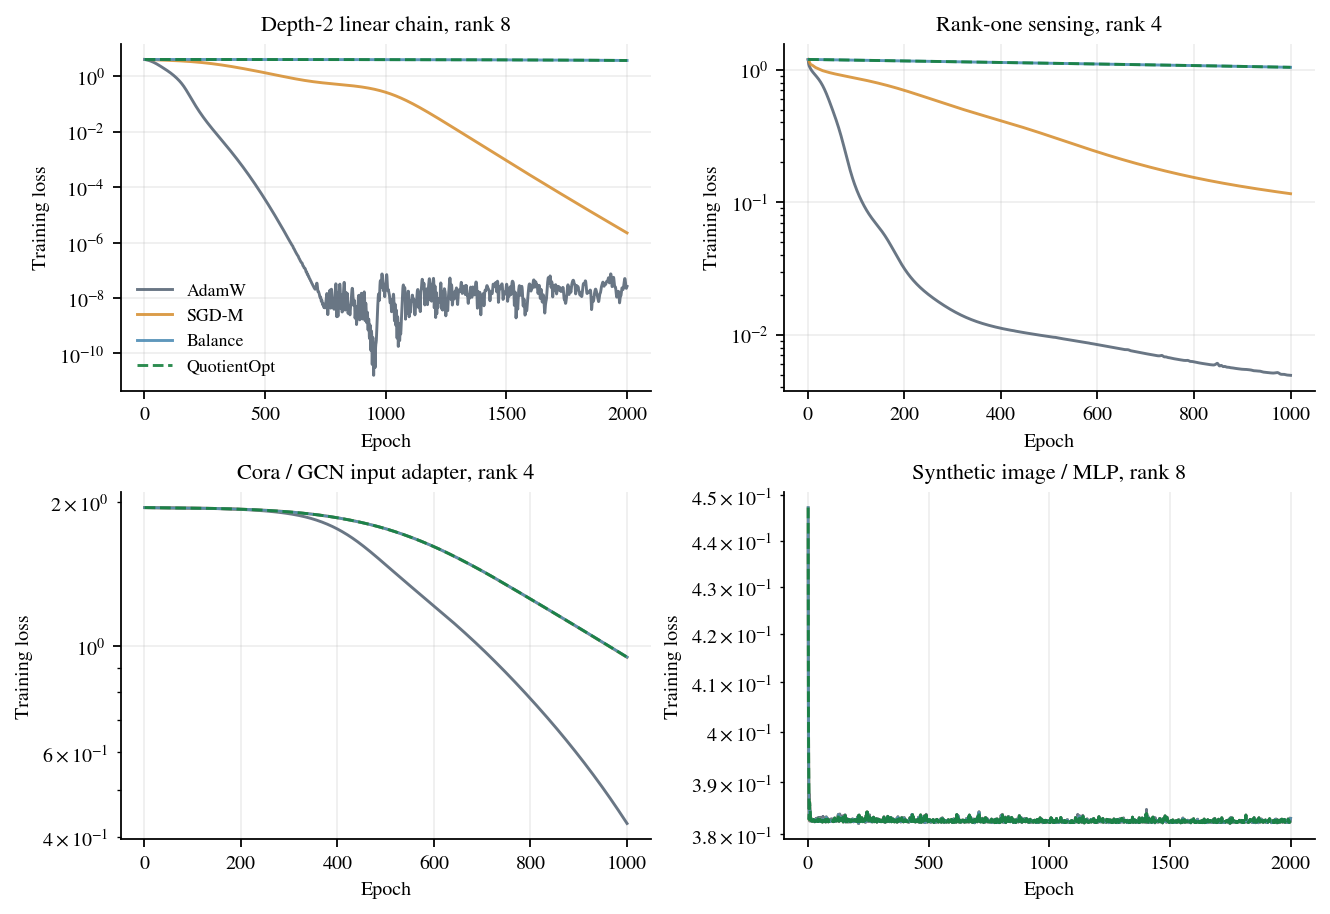
\includegraphics[width=.98\linewidth]{figures/replacement_trajectories.png}
\captionof{figure}{Initial completed central-setting replacement cohorts, before exhaustive tuning. The four panels show all four families with a matched completed cohort at the figure snapshot: 2000 epochs for depth-2 chains, sensing, and INR; 1000 epochs for Cora. The balanced momentum methods nearly overlap. AdamW optimizes the chain and sensing objectives much better at this setting; lower training loss on Cora does not imply higher test accuracy. These trajectories do not establish a best-tuned-method comparison.}
\label{fig:replacement-curves}

\end{minipage}\par\medskip

\paragraph{Central-setting outcomes across families.} At the displayed central setting, Cora/GCN's final test accuracy is $69.9\%$ for balance-only and QuotientOpt, versus $66.5\%$ for AdamW and $70.2\%$ for SGD-M. This is a positive comparison against AdamW, not against the stronger SGD-M endpoint. On the initial rank-one sensing and depth-2 chain cohorts, AdamW has substantially smaller final reconstruction error than the balanced momentum arms. The initial INR/MLP cohort has nearly tied held-out error across all four methods. Figure~\ref{fig:replacement-curves} reports the corresponding complete training trajectories. The search remains incomplete, so these are scoped central-setting outcomes, not conclusions from the full learning-rate/momentum/rank grid.
